\section{Results}\label{sec:results}
\subsection{Does SCC restore coverage under regime transfer?}\label{sec:res-cov}
At $\eta=0$, calibrating on one temperature and deploying on another, naive conformal miscovers
badly: coverage collapses to 0.572 when calibrating on short-lived and deploying on long-lived
units (a gap of 0.328), and over-covers wastefully in the reverse direction, reaching 1.000. In
maintenance terms, a 0.328 gap means roughly a third of the intervals promised at 90\% reliability
fail to contain the true life, an unsafe basis for a replacement decision. SCC holds every
calibrate--deploy pair between 0.891 and 0.908, so no pair falls more than 0.009 below the 0.90
target, for a mean coverage gap of 0.011 (Fig.~\ref{fig:cov}), and the non-exchangeable bound
$2\,\dtv(\tilde{\mathcal V})$ contains the SCC gap on every pair. The dimensionless transform removes
the $10.2\times$ scale difference exactly, the behaviour the zero-departure case of~\eqref{eq:cert}
predicts.

\begin{figure}[t]\centering
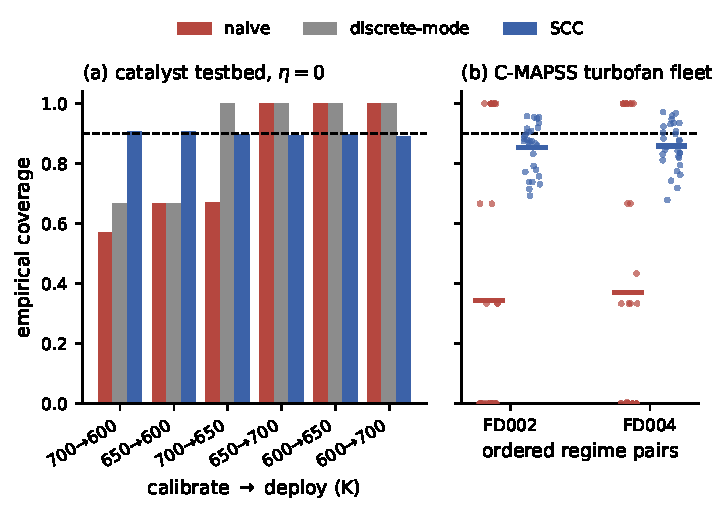
\includegraphics[width=\linewidth]{figures/fig1_coverage.pdf}
\caption{Naive vs.\ SCC coverage at $\eta=0$ across calibrate$\to$deploy temperature pairs, under
unit-level calibration. Naive miscovers (0.572) or over-covers (1.000); SCC tracks the 0.90 target
(0.891--0.908).}\label{fig:cov}
\end{figure}

\subsection{How does the guarantee degrade as physics departs from similitude?}\label{sec:res-deg}
As the unmodelled secondary channel is weighted up, the SCC coverage gap rises monotonically (0.011
at $\eta=0$ to 0.097 at $\eta=2$) and the interval back-off grows from 0.283 to 1.011
(Fig.~\ref{fig:dep}). Coverage is preserved at a quantified cost in conservatism, but that cost is
not uniformly benign: a back-off of 1.011 at $\eta=2$ means the certified lower bound is no longer
positive on average, so the interval remains valid while carrying no replacement schedule.
Reporting efficiency alongside coverage is what exposes this, instead of leaving a healthy-looking
coverage number to stand on its own.

\begin{figure}[t]\centering
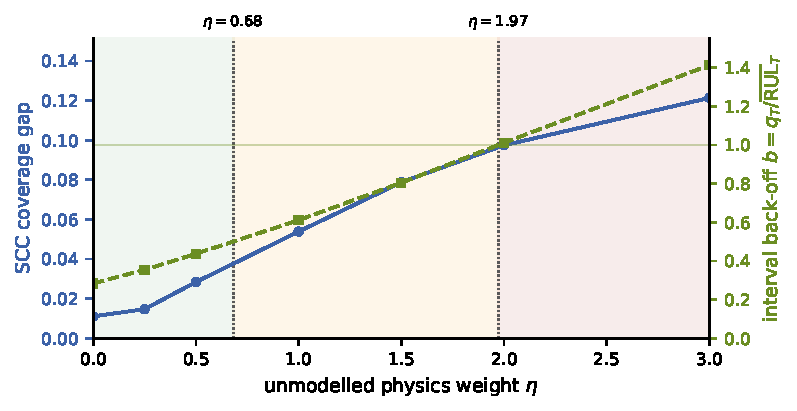
\includegraphics[width=\linewidth]{figures/fig2_departure.pdf}
\caption{Under a controlled departure $\eta$ from similitude, the SCC coverage gap (left axis) and
the relative interval back-off (right axis) degrade monotonically. The back-off reaches 1.011 at
$\eta=2$, where the certified lower bound is no longer positive on average.}\label{fig:dep}
\end{figure}

\subsection{Is the coverage bound reliable before deployment?}\label{sec:res-cert}
With the intercept $a$ and slope $L$ fit on 60\% of (pair, $\eta$) configurations, the physical
departure $\delta=\eta\lvert h(S)-h(T)\rvert$ predicts the dimensionless score-distribution mismatch
on the held-out 40\% with $R^2=0.773$ (correlation 0.947), and the resulting a-priori bound
$2(a+L\delta)$ upper-bounds the measured coverage gap on \emph{100\%} of held-out configurations
(Fig.~\ref{fig:cert}). Validity is not sharpness, and the margin says which one this is: across
held-out configurations the mean certified bound is 0.384 against a mean measured gap of 0.046, a
margin of 0.339 (range 0.268--0.552), so the certificate is conservative by roughly a factor of
eight. The looseness sits in the intercept rather than the physical slope, since at $\delta=0$ the
bound is $2a=0.278$ against a measured gap of 0.011. That intercept is the finite-sample floor of
the plug-in total-variation estimator and decays as $n^{-1/2}$ in the number of calibration units
(0.424 at 50 units to 0.096 at 800, a log-log slope of $-0.513$ against the $-0.500$ predicted), so
the certificate tightens as the calibration fleet grows. For deployment this means the worst-case
coverage shortfall can be quoted from physical parameters before the target asset is run, as a
worst-case planning bound rather than a sharp estimate.

\begin{figure}[t]\centering
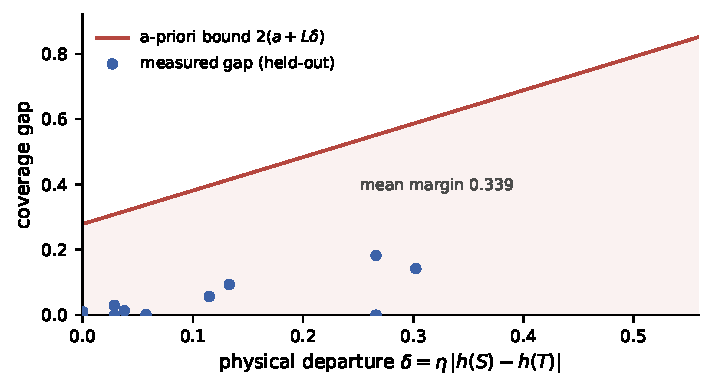
\includegraphics[width=\linewidth]{figures/fig3_certificate.pdf}
\caption{Held-out measured coverage gap vs.\ the physical departure $\delta$, with the a-priori bound
$2(a+b\delta)$ fit on disjoint configurations. The bound holds on 100\% of held-out
points.}\label{fig:cert}
\end{figure}

\subsection{Robustness across operating and tuning choices}\label{sec:res-rob}
The acceptance criteria survive across the departure's temperature-dependence ($E_2=95$--150~kJ/mol
at matched magnitude), its magnitude (15--60\% perturbation), and the coverage target
($\alpha=0.05/0.10/0.20$); Table~\ref{tab:robust}. At every setting naive conformal miscovers
($\approx0.13$), SCC recovers ($\approx0.011$), the a-priori bound holds on 100\% of held-out
configurations while carrying a margin of 0.30--0.50, the same conservatism reported in
Section~\ref{sec:res-cert}, the gap stays monotone, and its magnitude orders with the steepness and
size of the departure. The behaviour is a property of the method rather than of a single tuning.

\begin{table}[t]\centering\footnotesize
\setlength{\tabcolsep}{9pt}\renewcommand{\arraystretch}{1.2}
\caption{Robustness of the acceptance criteria across the departure's temperature-dependence, its
magnitude, and the coverage level, under unit-level calibration. $g_0$: coverage gap at $\eta=0$;
$g_{\max}$: SCC coverage gap at $\eta=2$; Margin: mean of (certified bound $-$ measured gap) over
held-out configurations, so a positive value means valid and a large value means loose; Bound\,\%:
fraction of held-out configurations on which the a-priori bound holds.}\label{tab:robust}
\begin{tabular}{@{}llccccc@{}}\toprule
Perturbation axis & Value & Naive $g_0$ & SCC $g_0$ & SCC $g_{\max}$ & Margin & Bound\,\% \\\midrule
$E_2$ (kJ/mol) & 95   & 0.132 & 0.011 & 0.043 & 0.302 & 100 \\
               & 150  & 0.132 & 0.011 & 0.218 & 0.502 & 100 \\
Perturbation   & 15\,\% & 0.132 & 0.011 & 0.055 & 0.302 & 100 \\
               & 60\,\% & 0.132 & 0.011 & 0.131 & 0.400 & 100 \\
Coverage $\alpha$ & 0.05 & 0.138 & 0.008 & 0.071 & 0.372 & 100 \\
               & 0.20 & 0.103 & 0.011 & 0.127 & 0.323 & 100 \\\bottomrule
\end{tabular}
\end{table}

\subsection{Knowing when not to trust the method: the diagnostic on a thin experimental benchmark}\label{sec:res-diag}
On synthetic data the runtime diagnostic discriminates correctly: it returns \emph{holds} when lives
obey L10, \emph{violated} when they do not (with adequate units), and \emph{indeterminate} when the
within-condition spread swamps the structural signal (Fig.~\ref{fig:diag}). The FEMTO bearing
benchmark~\cite{nectoux2012pronostia} is an accelerated laboratory test platform, not field data
from an operating fleet, and it falls in the last category: with roughly six bearings per
condition and a $7\times$ within-condition life spread, the bootstrap CI on $g$ spans a factor of
2.6--4.4, far too wide to resolve the $1.63\times$ life ratio that L10 predicts between its load/speed
conditions. The diagnostic therefore returns \emph{indeterminate} and SCC declines its a-priori
certificate, deferring to data-driven conformal. This is an honest applicability limit rather than a
failure, and it is consistent with the dataset authors' report that L10 does not govern FEMTO lives;
it also shows the diagnostic doing its safety job, refusing to certify on evidence too weak to
support the premise.

\begin{figure}[t]\centering
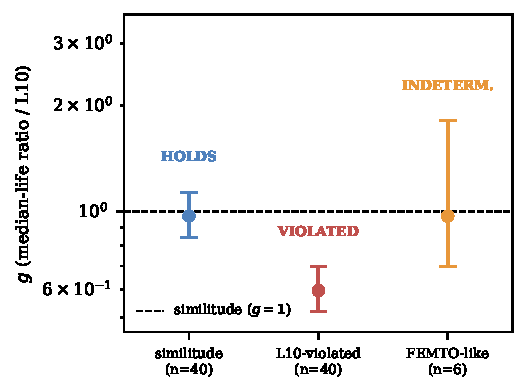
\includegraphics[width=\linewidth]{figures/fig4_diagnostic.pdf}
\caption{Diagnostic verdict via bootstrap CIs on $g$ (median-life ratio normalised by the L10
prediction; $g{=}1$ under similitude). Synthetic similitude $\to$ holds; powered violation $\to$
violated; FEMTO-like (few units, large spread) $\to$ indeterminate.}\label{fig:diag}
\end{figure}
